\documentclass{standalone}\usepackage{pgfplots}\pgfplotsset{compat=1.18}\begin{document}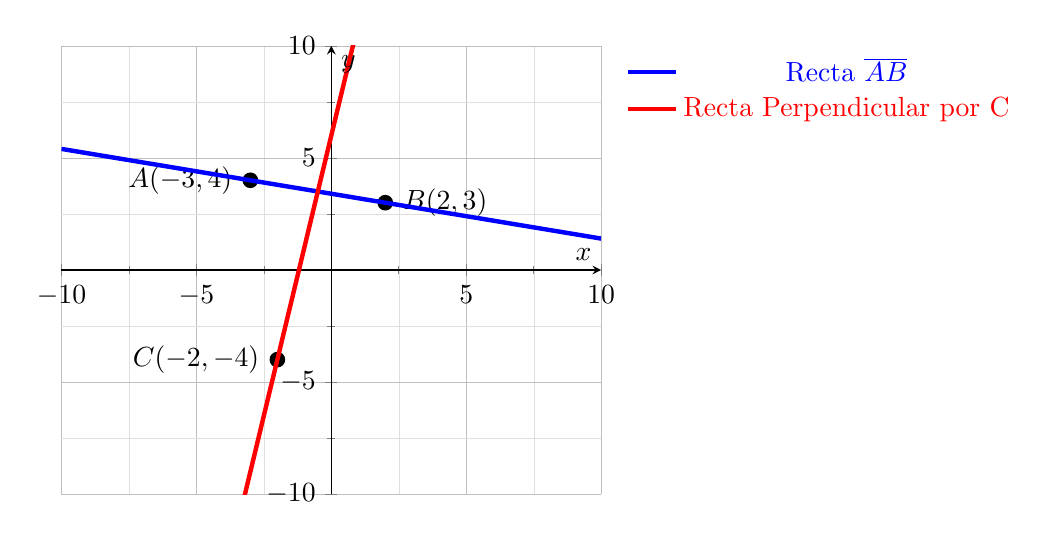
\begin{tikzpicture}
\begin{axis}[
    axis lines = middle,
    xlabel = \( x \),
    ylabel = \( y \),
    xmin=-10, xmax=10,
    ymin=-10, ymax=10,
    grid=both,
    minor tick num=1,
    major grid style={line width=.2pt,draw=gray!50},
    minor grid style={line width=.1pt,draw=gray!25},
    samples=100,
    legend pos=outer north east,
    legend style={draw=none},
]

% Dibujar puntos A, B y C con etiquetas
\node[label={180:{\( A(-3,4) \)}},circle,fill,inner sep=2pt] at (axis cs:-3,4) {};
\node[label={0:{\( B(2,3) \)}},circle,fill,inner sep=2pt] at (axis cs:2,3) {};
\node[label={180:{\( C(-2,-4) \)}},circle,fill,inner sep=2pt] at (axis cs:-2,-4) {};

% Dibujar recta AB
\addplot[domain=-10:10, blue, ultra thick] {-1/5*x + 17/5};
\addlegendentry{\textcolor{blue}{Recta $\overline{AB}$}}

% Dibujar recta perpendicular por C
\addplot[domain=-10:10, red, ultra thick] {5*x + 6};
\addlegendentry{\textcolor{red}{Recta Perpendicular por C}}

\end{axis}
\end{tikzpicture}\end{document}